\documentclass[12pt,a4paper,dvipdfmx]{jarticle}
%
\topmargin=-5mm
\oddsidemargin=-5mm
\evensidemargin=-5mm
\textheight=235mm
\textwidth=165mm
%
\title{FDPS講習会の手引 (Fortran版)}
\author{行方大輔、谷川衝、岩澤全規、細野七月、似鳥啓吾、村主崇行、野村昴太郎、 \\ 坪内美幸、牧野淳一郎}
\date{\today}
%\pagestyle{empty}
\usepackage[dvipdfmx]{graphicx}
\usepackage{wrapfig}
\usepackage{lscape}
\usepackage{amssymb}
\usepackage{amsmath}
\usepackage{bm}
\usepackage{setspace}
%\usepackage{listings,jlisting}
\usepackage{color}
\usepackage{ascmac}
\usepackage{here}
\usepackage[dvipdfmx]{hyperref}
\usepackage{pxjahyper}

\newcommand{\underbold}[1]{\underline{\bf #1}}
\newcommand{\redtext}[1]{\textcolor{red}{#1}}

%\setcounter{secnumdepth}{4}
%%%%%%%%%%%%%%%%%%%%%%%%%%%%%%%%%%
\setcounter{secnumdepth}{5}
\makeatletter
\newcommand{\subsubsubsection}{\@startsection{paragraph}{4}{\z@}%
{1.5\baselineskip \@plus.5\dp0 \@minus.2\dp0}%
{.5\baselineskip \@plus2.3\dp0}%
{\reset@font\normalsize\bfseries}
}
\newcommand{\subsubsubsubsection}{\@startsection{subparagraph}{5}{\z@}%
{1.5\baselineskip \@plus.5\dp0 \@minus.2\dp0}%
{.5\baselineskip \@plus2.3\dp0}%
{\reset@font\normalsize\itshape}
}
\makeatother
\setcounter{tocdepth}{5}
%%%%%%%%%%%%%%%%%%%%%%%%%%%%%%%%%%

\begin{document}
\maketitle
\tableofcontents

\newpage





\section{準備}


\subsection{自分で用意した計算機で実行する場合}
\texttt{https://github.com/FDPS/FDPS}からFDPSの最新版をダウンロードし、好きな
ディレクトリ下で解凍する。これによってディレクトリ\texttt{FDPS-master}が出来る。


以下の方法のいずれかでFDPSの最新バージョンを取得できる。
\begin{itemize}
\item ブラウザから
  \begin{enumerate}
  \item ウェブサイト \url{https://github.com/FDPS/FDPS}で"Download ZIP"をクリックし、ファイル\path{FDPS-master.zip}をダウンロード
  \item FDPSを展開したいディレクトリに移動し、圧縮ファイルを展開
  \end{enumerate}

\item コマンドラインから
  \begin{itemize}    
  \item Subversionを用いる場合:以下のコマンドを実行するとディレクトリ
    trunkの下をSubversionレポジトリとして使用できる
    \begin{screen}
\begin{verbatim}
$ svn co --depth empty https://github.com/FDPS/FDPS
$ cd FDPS
$ svn up trunk
\end{verbatim}
    \end{screen}

  \item Gitを用いる場合:以下のコマンドを実行するとカレントディレクト
    リにディレクトリFDPSができ、その下をGitのレポジトリとして使用できる
    \begin{screen}
\begin{verbatim}
$ git clone git://github.com/FDPS/FDPS.git
\end{verbatim}
    \end{screen}    

  \end{itemize}

\end{itemize}


以下では、ウェブサイトからダウンロードした場合を想定し、ディレクトリ\texttt{FDPS-master}があるディレクトリの名前を\texttt{fdps}とする。

\section{実習本番}

実習で行うことは、FDPSを使って実装された重力$N$体シミュレーションコード
とSPHシミュレーションコードを使用することである。最初に重力$N$体シミュ
レーションコード、次にSPHシミュレーションコードを使用する。

なお、実習の際に\texttt{Makefile}を更新し、コンパイルし直すという作業を
何回か行うが、ここで注意しなくてはならないのは、
\textbf{\texttt{Makefile}を編集しただけでは実行ファイルの再作成は行われ
  ない}ということである。この場合、きちんと前回作った実行ファイルを明示
的に``\texttt{\$ rm ./nbody.out}''などで消す必要がある。これを忘れた場
合、「\texttt{make: `nbody.out'} は更新済みです」と出る。

\subsection{重力$N$体シミュレーションコード}
ここでは、重力$N$体シミュレーションコードでのcold collapseを、
並列環境無し、OpenMPを用いた並列計算環境、OpenMP + MPIを用いた並列計算環境の3つで行う。
MPI は、環境があれば行う。

%\color{red}
%そのためにはこういう事をします云々。。。
%\color{black}

\subsubsection{概要}

ここでは、用意された重力$N$体シミュレーションコードを動かしてみよう。こ
のコードは、重力多体系のコールドコラプスを計算する。この節でまず行うこ
とは、シリアルコードのコンパイルと実行、出て来た結果の解析である。次に
シリアルコードをPhantom-GRAPEを用いて高速化して、その速さを体験しよう。
最後にOpenMPやMPI を利用して、さらにコードを高速化する。

\subsubsection{シリアルコード}

以下の手順で本コードを使用できる。
\begin{itemize}
\item ディレクトリ\texttt{fdps/FDPS-master/sample/fortran/nbody}に移動
\item \texttt{make}を実行
\item ジョブの投入
\item 結果の解析
\item OpenMP/MPIの利用(オプション)
\end{itemize}

\subsubsubsection{ディレクトリ移動}

ディレクトリ\texttt{fdps/FDPS-master/sample/fortran/nbody}に移動する。
\begin{screen}
\begin{verbatim}
$ cd fdps/FDPS-master/sample/fortran/nbody
\end{verbatim}
\end{screen}

\subsubsubsection{makeの実行}
\texttt{make}コマンドを実行する。
\begin{screen}
\begin{verbatim}
$ make
\end{verbatim}
\end{screen}

\subsubsubsection{計算の実行}

まずは、インタラクティブ実行で計算を実行する。これは、生成された実行ファ
イルの名前をそのまま実行すればよい。
\begin{screen}
\begin{verbatim}
$ ./nbody.out
\end{verbatim}
\end{screen}

正しくジョブが終了すると、標準入出力の最後には以下のようなログが出力さ
れるはずである。energy errorは絶対値で$1 \times 10^{-3}$のオーダーに収
まっていればよい。
\begin{screen}
\begin{verbatim}
time:    9.5000000000E+000, energy error:   -3.5093659762E-003
time:    9.6250000000E+000, energy error:   -3.5829042035E-003
time:    9.7500000000E+000, energy error:   -3.6160022980E-003
time:    9.8750000000E+000, energy error:   -3.5109567381E-003
******** FDPS has successfully finished. ********
\end{verbatim}
\end{screen}
ただし、後述するPhantom-GRAPEを用いた場合、energy error数値は変わるので注意する。

\subsubsubsection{結果の解析}

ディレクトリ\texttt{result}に粒子分布を出力したファイル
"snap000\textit{xx}-prc000\textit{yy}.dat"ができている。
\textit{xx}、\textit{yy}はいずれも0埋めされた整数で、
前者は時刻を、後者はMPIのランク番号(逐次実行の場合には必ず0となる)を表す。
出力ファイルフォーマットは1列目から順に粒子のID, 粒子の質量、位置の$x$,
$y$, $z$座標、粒子の$x$, $y$,$z$軸方向の速度である。

ここで実行したのは、粒子数1024個からなる一様球(半径3)のコールドコラプス
である。コマンドライン上で以下のコマンドを実行すれば、時刻9における
$xy$平面に射影した粒子分布を見ることができる。
\begin{screen}
\begin{verbatim}
$ gnuplot
$ plot "result/snap00009-proc00000.dat" using 3:4
\end{verbatim}
\end{screen}

他の時刻の粒子分布をプロットすると、一様球が次第に収縮し、その後もう一
度膨張する様子を見ることができる(図\ref{fig:nbody}参照)。

\begin{figure}
  \begin{center}
        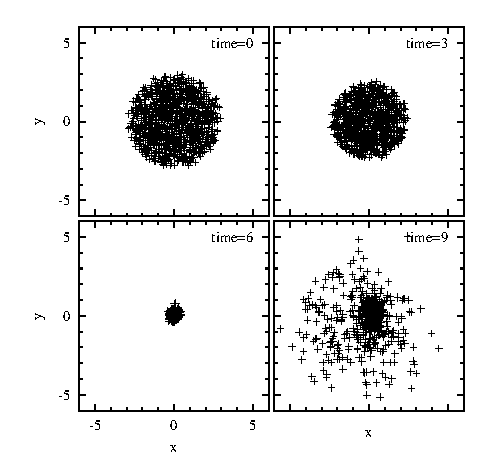
\includegraphics[width=10cm,bb=0 0 220 220]{fig/nbody.eps}
  \end{center}
  \caption{}
  \label{fig:nbody}
\end{figure}

\subsubsection{Phantom-GRAPEの利用}

以下では、相互作用計算にPhantom-GRAPEを使う場合について、記述する。この
場合、ユーザーはまずはPhantom-GRAPE用の\texttt{Makefile}を利用環境
(使用するコンパイラ等)に合わせて適切に変更する必要がある。
今回使うPhantom-GRAPEのソースコードは、
\texttt{fdps/FDPS-master/src/phantom\_grape\_x86/G5/newton/libpg5/} 以
下に存在するので、そこまで移動し、\texttt{Makefile}を編集する。以下は、現在
\texttt{sample/fortran/nbody/}に居る場合の例である。
\begin{screen}
\begin{verbatim}
$ cd ../../../src/phantom_grape_x86/G5/newton/libpg5/
$ vi Makefile
\end{verbatim}
\end{screen}

編集が終わったら、元のディレクトリに戻る(サンプルコード側の\texttt{Makefile}で自動的にPhantom-GRAPEライブラリをビルドする設定になっているので、ここでコンパイルする必要はない)。
次に、\texttt{Makefile}の修正を行う。\texttt{Makefile}の34行目に
Phantom-GRAPEを使用するか否かを決定しているスイッチが存在している。この
スイッチはデフォルトではコメントアウトされているため、
以下のようにしてコメントアウトを解除する。
\begin{screen}
\begin{verbatim}
use_phantom_grape_x86 = yes
\end{verbatim}
\end{screen}

無事にコンパイルが通れば、以降の実行・解析の手順は同様である。実行直後
に次のような表示がされれば、正しく実行ができている。
\begin{screen}
\begin{verbatim}
******** FDPS has successfully begun. ********
====================================
 Paralleization infomation:
   # of processes is 1
   # of thread is    1
====================================
rsqrt: MSE = 1.158186e-04,  Bias = 8.375360e-08
(以下省略)
\end{verbatim}
\end{screen}

\subsubsection{PIKGの利用}

以下では、PIKGで生成された相互作用計算カーネルを使う場合について記述する。
まず\texttt{Makefile}の修正を行う。\texttt{Makefile}の35行目に
PIKGを使用するか否かを決定しているスイッチが存在している。このスイッチは
デフォルトではコメントアウトされているため、以下のようにしてコメントアウトを解除する。
\begin{screen}
\begin{verbatim}
use_pikg_x86 = yes
\end{verbatim}
\end{screen}

\texttt{make}を実行し無事にコンパイルが通れば、以降の実行・解析の手順は同様である。

\subsubsection{OpenMP/MPIの利用}

OpenMPやMPIを利用する場合について以下に記述する。

\begin{itemize}
\item OpenMPのみ使用の場合
  \begin{itemize}
  \item \texttt{Makefile}の編集
    \begin{itemize}
    \item マクロ\texttt{FC}, \texttt{CXX}に、それぞれOpenMP対応のFortran, C++コンパイラを代入する。
        \item ``\texttt{FCFLAGS += -DPARTICLE\_SIMULATOR\_THREAD\_PARALLEL -fopenmp}''の行のコメントアウトを外す
    \item ``\texttt{CXXFLAGS += -DPARTICLE\_SIMULATOR\_THREAD\_PARALLEL -fopenmp}''の行のコメントアウトを外す
    \end{itemize}
  \item 環境変数 \texttt{OMP\_NUM\_THREADS} の値を使用したいスレッド数にする。利用環境がLinux あるいは UNIXで、シェルが\text{bash}の場合、スレッド数を4に設定するには以下を実行する。
\begin{screen}
\begin{verbatim}
$ export OMP_NUM_THREADS = 4
\end{verbatim}
\end{screen}
  \item \texttt{make}コマンドを実行する。
  \item 実行方法はシリアルコードの場合と同じである。

\begin{screen}
\begin{verbatim}
(省略)
******** FDPS has successfully begun. ********
====================================
 Paralleization infomation:
   # of processes is 1
   # of thread is    4
====================================
(以下省略)
\end{verbatim}
\end{screen}
       \texttt{\# of thread is    4}と表示されている。
       これで、4スレッドでの並列計算が行われている事が確認できた。
\end{itemize}

\item OpenMPとMPIの同時使用の場合
  \begin{itemize}
  \item \texttt{Makefile}の編集
    \begin{itemize}
    \item マクロ\texttt{FC}, \texttt{CXX}に、それぞれMPI対応のFortran, C++コンパイラを代入する。
    \item ``\texttt{FCFLAGS += -DPARTICLE\_SIMULATOR\_THREAD\_PARALLEL -fopenmp}''の
      行のコメントアウトを外す
    \item ``\texttt{CXXFLAGS += -DPARTICLE\_SIMULATOR\_THREAD\_PARALLEL -fopenmp}''の
      行のコメントアウトを外す
    \item ``\texttt{FCFLAGS += -DPARTICLE\_SIMULATOR\_MPI\_PARALLEL}''の行のコメントアウトを外す
    \item ``\texttt{CXXFLAGS += -DPARTICLE\_SIMULATOR\_MPI\_PARALLEL}''の行のコメントアウトを外す
    \end{itemize}
  \item 環境変数 \texttt{OMP\_NUM\_THREADS} の値を使用したいスレッド数に設定する。
  \item \texttt{make}コマンドを実行する。
  \item システムの MPI 環境の方法で実行する。(例えば、 mpirun -np 2
    ./nbody.out) 正しく実行された場合、以下のように表示されるはずである。
\begin{screen}
\begin{verbatim}
(省略)
******** FDPS has successfully begun. ********
====================================
 Paralleization infomation:
   # of processes is 2
   # of thread is    2
====================================
(以下省略)
\end{verbatim}
\end{screen}
       \texttt{\# of processes is 2}、\texttt{\# of thread is    2}と表示されており、2プロセス2スレッドでの並列計算が行われている事が確認できた。
\end{itemize}
\end{itemize}

\subsection{SPHシミュレーションコード}

\subsubsection{概要}

ここでは、SPHシミュレーションコードを動かす。用意されているコードは、
衝撃波管問題の計算を行う。この節でまず行うことは、シリアルコード
のコンパイルと実行、出て来た結果の解析である。最後にOpenMPやMPI を利用
して、さらにコードを高速化する。

\subsubsection{シリアルコード}

以下の手順で本コードを使用できる。
\begin{itemize}
\item ディレクトリ\texttt{fdps/FDPS-master/sample/fortran/sph}に移動
\item \texttt{make}を実行
\item ジョブの投入
\item 結果の解析
\item OpenMP/MPIの利用(オプション)
\end{itemize}

\subsubsubsection{ディレクトリ移動}

ディレクトリ\texttt{fdps/FDPS-master/sample/fortran/sph}に移動する。

\subsubsubsection{makeの実行}

\texttt{make}コマンドを実行する。

\subsubsubsection{計算の実行}
まずは、インタラクティブ実行で計算を実行する。
これは、生成された実行ファイルの名前をそのまま実行すればよい。
\begin{screen}
\begin{verbatim}
$ ./sph.out
\end{verbatim}
\end{screen}

正しくジョブが終了すると、標準入出力の最後には以下のようなログが出力されるはずである。
\begin{screen}
\begin{verbatim}
(省略)
================================
time  =   1.1809149264408111E-001
nstep =     54
================================
================================
time  =   1.2037329341359981E-001
nstep =     55
================================
******** FDPS has successfully finished. ********
STOP 0
\end{verbatim}
\end{screen}

\subsubsubsection{結果の解析}

ディレクトリ\texttt{result}にファイルが出力されている。
ファイル名は"snap000\textit{xx}-proc00\textit{yy}.dat"となっている。
\textit{xx}, \textit{yy}は0埋めされた整数で、前者が時刻を、
後者がMPIのランク番号を表す。出力ファイルフォーマットは1列目から順に
粒子のID、粒子の質量、位置の$x$, $y$, $z$ 座標、粒子の
$x$, $y$, $z$軸方向の速度、密度、内部エネルギー、圧力である。

以下のコマンドを実行すれば、横軸に$x$、縦軸に密度の図が作成される。

\begin{screen}
\begin{verbatim}
$ gnuplot
> plot "result/snap0040-proc00000.dat" using 3:9 w p
\end{verbatim}
\end{screen}
正しい答が得られれば、図\ref{fig:sph_ftn}のような図を描ける。

\begin{figure}
  \begin{center}
    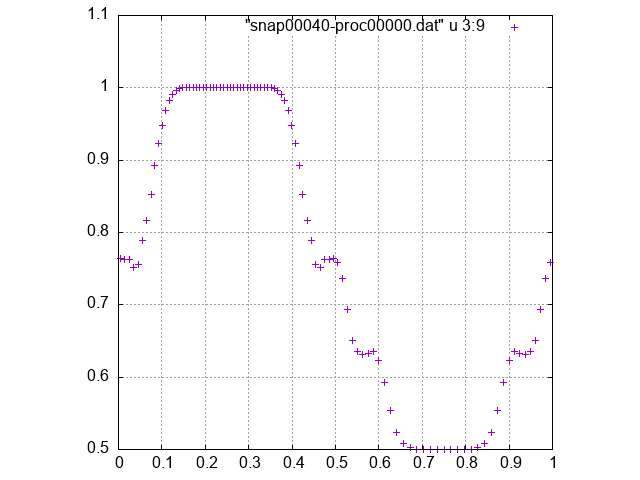
\includegraphics[width=10cm]{fig/sph_ftn.png}
  \end{center}
  \caption{}
  \label{fig:sph_ftn}
\end{figure}

\subsubsection{OpenMP/MPIの利用}

OpenMPやMPIを利用する場合を以下に示す。
\begin{itemize}
\item OpenMPのみ使用の場合
  \begin{itemize}
  \item \texttt{Makefile}の編集
    \begin{itemize}
    \item マクロ\texttt{FC}, \texttt{CXX}に、それぞれOpenMP対応のFortran, C++コンパイラを代入する
    \item ``\texttt{FCFLAGS += -DPARTICLE\_SIMULATOR\_THREAD\_PARALLEL -fopenmp}''の行のコメントアウトを外す
    \item ``\texttt{CXXFLAGS += -DPARTICLE\_SIMULATOR\_THREAD\_PARALLEL -fopenmp}''の行のコメントアウトを外す
    \end{itemize}
  \item 環境変数 \texttt{OMP\_NUM\_THREADS} の値を使用したいスレッド数にする。
  \item \texttt{make}コマンドを実行する。
  \item シリアルコードと同じように実行する。正しく実行された場合、以下のように表示されるはずである。
\begin{screen}
\begin{verbatim}
******** FDPS has successfully begun. ********
====================================
 Paralleization infomation:
   # of processes is 1
   # of thread is    2
====================================
\end{verbatim}
\end{screen}
  \end{itemize}

\item OpenMPとMPIの同時使用の場合
  \begin{itemize}
  \item \texttt{Makefile}の編集
    \begin{itemize}
    \item マクロ\texttt{FC}, \texttt{CXX}に、それぞれMPI対応のFortran, C++コンパイラを代入する
    \item ``\texttt{FCFLAGS += -DPARTICLE\_SIMULATOR\_THREAD\_PARALLEL -fopenmp}''の行のコメントアウトを外す
    \item ``\texttt{CXXFLAGS += -DPARTICLE\_SIMULATOR\_THREAD\_PARALLEL -fopenmp}''の行のコメントアウトを外す
    \item ``\texttt{FCFLAGS += -DPARTICLE\_SIMULATOR\_MPI\_PARALLEL}''の行のコメントアウトを外す
    \item ``\texttt{CXXFLAGS += -DPARTICLE\_SIMULATOR\_MPI\_PARALLEL}''の行のコメントアウトを外す
    \end{itemize}
  \item 環境変数 \texttt{OMP\_NUM\_THREADS} の値を使用したいスレッド数にする。
  \item \texttt{make}コマンドを実行する。
  \item システムの MPI 環境の使い方に従って実行する。正しく実行された場合、以下のように表示されるはずである。
\begin{screen}
\begin{verbatim}
******** FDPS has successfully begun. ********
====================================
 Paralleization infomation:
   # of processes is 2
   # of thread is    2
====================================
\end{verbatim}
\end{screen}
\end{itemize}
\end{itemize}

\end{document}
